\chapter{知識・技術習得}

\section{リスク分析}
%各人の担当課題の概要と，プロジェクト内における役割・位置づけを記述する．
プロジェクトを本格的に開始する前に，リスク分析を行った．各個人がプロジェクト活動で起こり得ると思う問題とその発生確率，発生した場合の被害，問題の対策について考えた．考えたものについてランダムに分かれたグループ内で発表し，グループ単位でGoogleスプレッドシートにまとめ，さらにそのスプレッドシートをもとに全体で1つのGoogleスプレッドシートにまとめた．その後奥野教授からフィードバックを頂き，今後の活動に役立つ共通知識を得ることができた．
\begin{figure}[H]
    \centering
    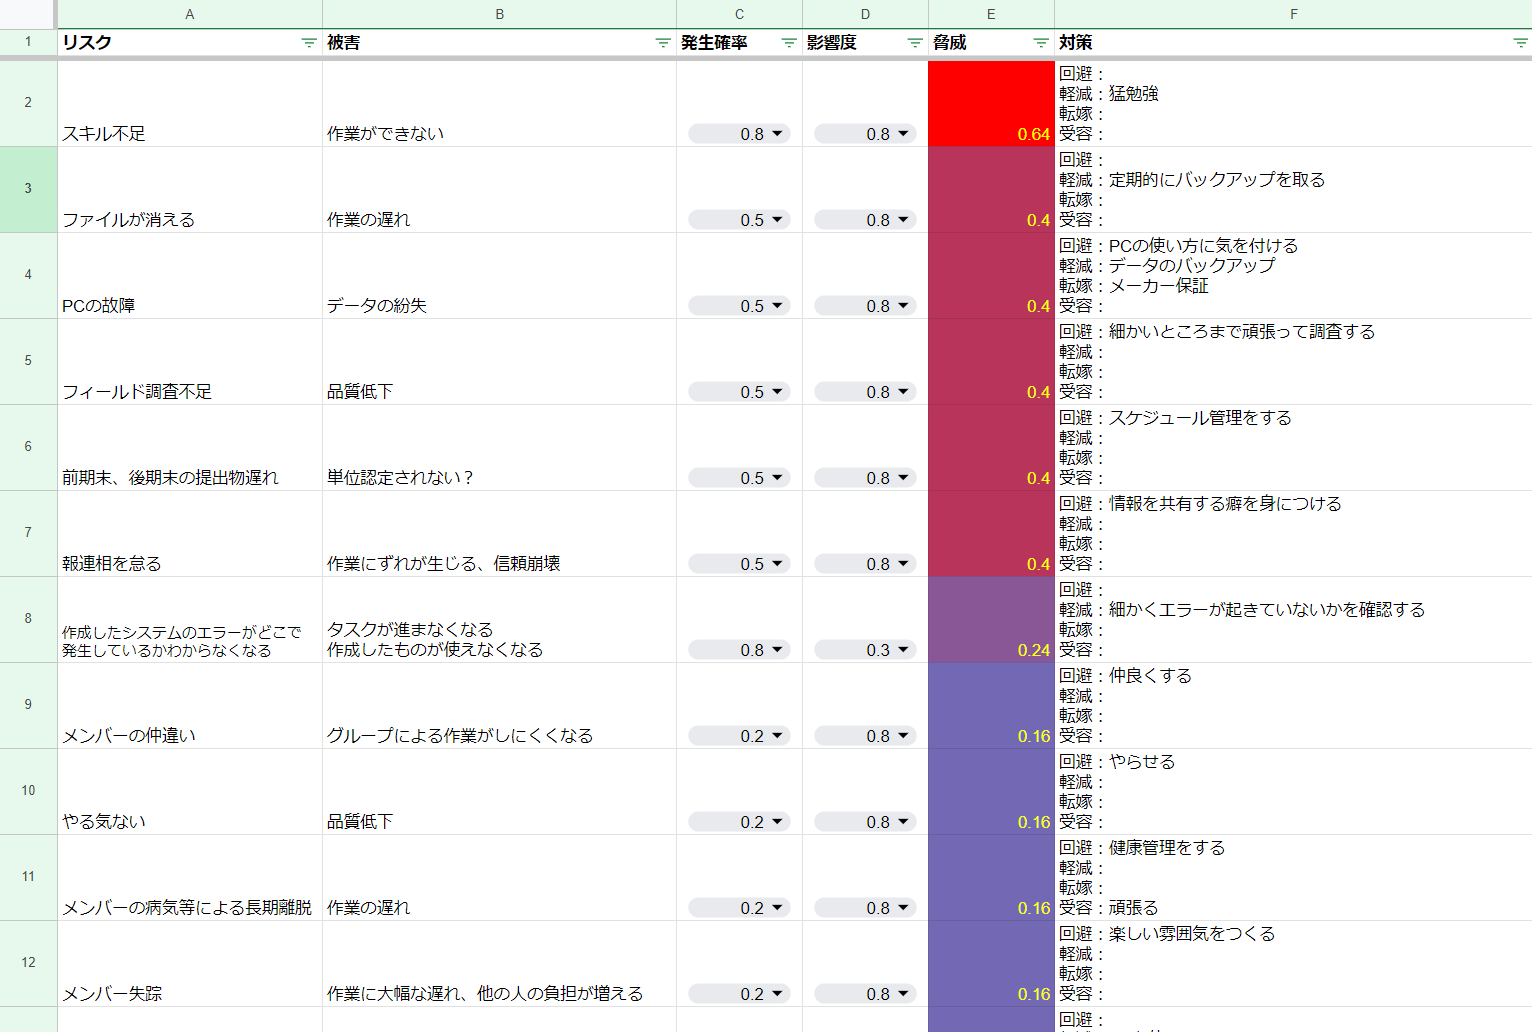
\includegraphics[width=12cm]{images/4.1_risk.png}
    \caption{リスク分析の抜粋}
    \figlab{risk}
\end{figure}
\bunseki{大須賀雅也}

\section{アジャイル開発概論 （enPiT e-Learning）}
プロジェクトの開始時に事前ビデオ教材「アジャイル開発概論（enPiT e-Learning）」の「プロジェクト学習のためのプロジェクトマネジメントの基礎」を視聴した．この学習を通じて，アジャイル開発の概念と原則について詳しく学んだ．プロジェクトマネジメントについては，プロジェクトを計画し，進行させるための方法論で，プロジェクト内での役割について学び，プロジェクトの成功に向けて必要な活動に取り組むことが重要である．具体的に，計画立案，リスク分析，スケジュール管理などの内容について詳細に学んだ．これらの知識を身につけることで，今後のプロジェクト学習活動において不可欠なスキルを獲得し，メンバー全員が共通の知識を持つことで，グループ活動を円滑に進めることが可能である．
\bunseki{高橋慧流}

\section{フィールドワーク入門講座}
フィールドワークがどのような活動なのか理解するため，5月31日に南部准教授と元木准教授による対面でのフィールドワーク入門講座を，プロジェクトメンバー全員で受講した．講座はスライド（図\ref{fig:field}）を用いて，そもそもフィールドワークとはなにか，実際に過去のフィールドワークではどのようなことを行い，どのような問題が発生したか，何に気をつけるべきか（注意事項）を教えていただいた．実際に現場に行って問題点や解決の糸口を見つけることの重要さや，ただ街をぶらぶらするのではなく社会や文化を知るために観察と記録を怠らないことが大事であるということを学んだ．
\begin{figure}[H]
    \centering
    \fbox{
    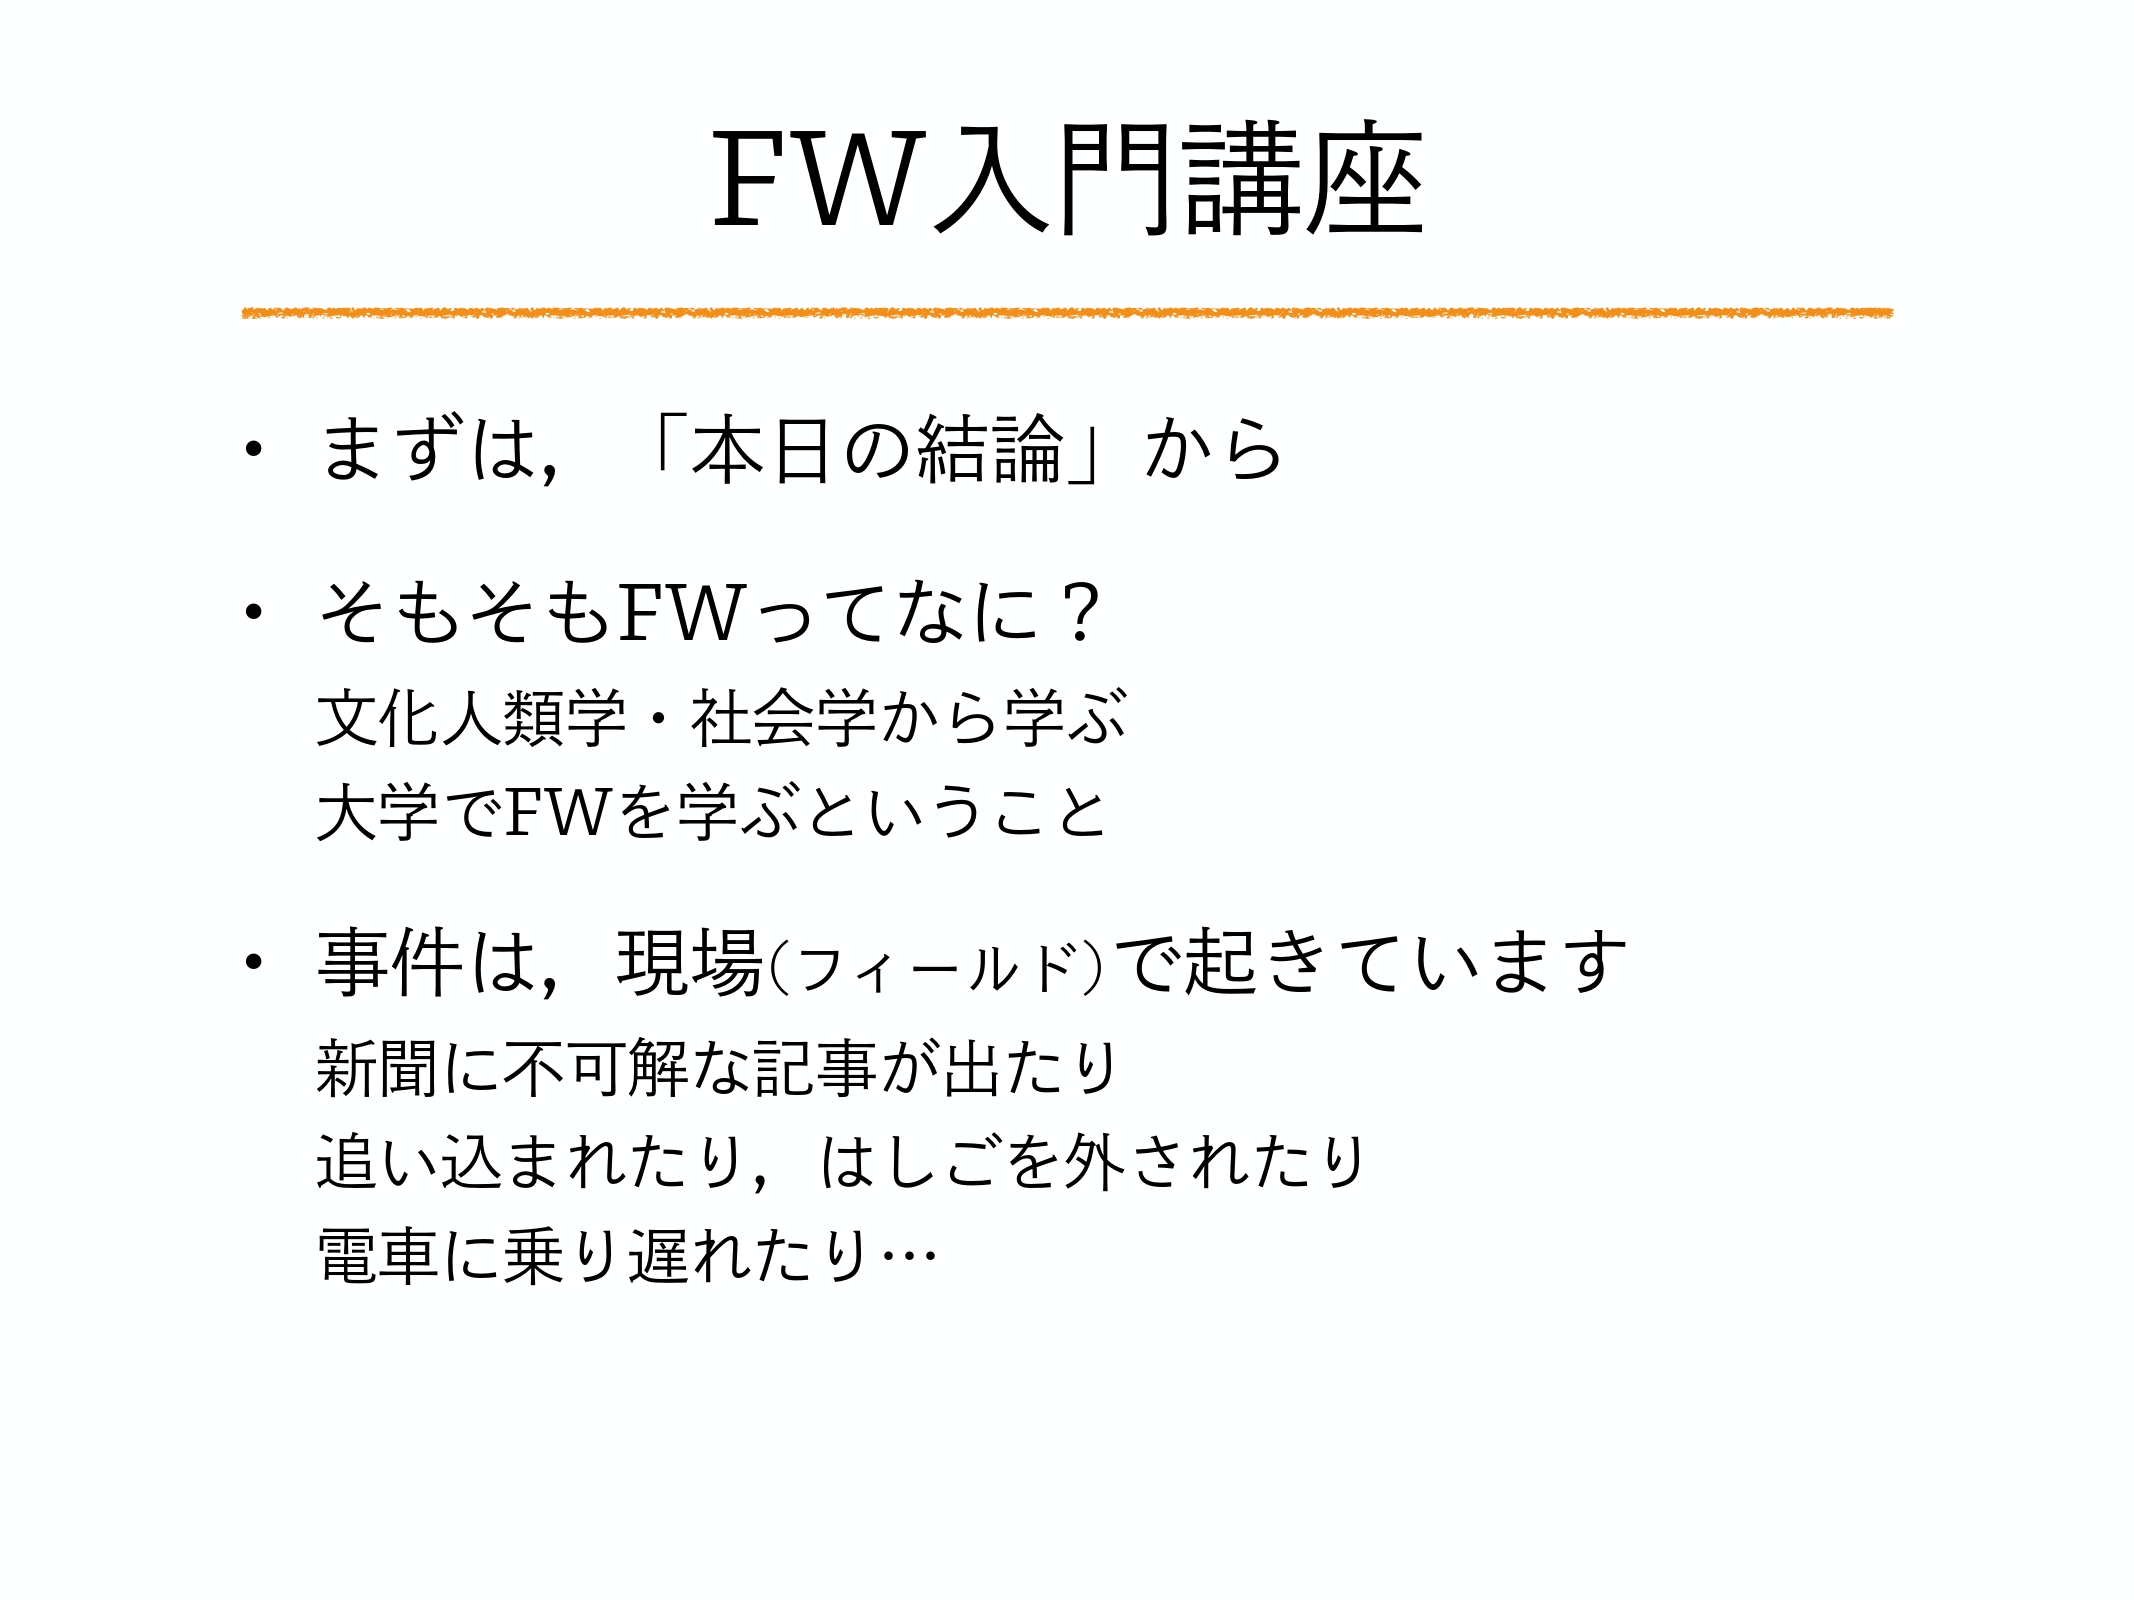
\includegraphics[width=8cm]{images/fieldwork.jpg}
    }
    \caption{フィールドワーク入門講座\cite{field}のスライドの一部}
    \figlab{field}
\end{figure}
\bunseki{齊藤輝}

\section{アジャイルワークショップ}

\subsection{DNPアジャイルワークショップ}
私達は5月29日に開催された大日本印刷株式会社主催のDNPアジャイルワークショップに参加した．大日本印刷株式会社が開発したアジャイル開発の流れについてがわかるボードゲームを学生同士で体験し，アジャイル開発とスクラムに関する知見を深めることができた．特に知識や技術を先に習得しておくことは後の開発をスムーズに進めることになり，非常に重要であることがわかった．
\bunseki{南川虎之介}

\subsection{アジャイルワークショップ}
私達は6月14日に株式会社アトラクタの永瀬美穂氏を講師に迎えて，アジャイルワークショップをプロジェクトメンバー全員で受講した．このワークショップでは，アジャイル開発についての知識をさらに深める機会を得た．ワークショップの前半では，ビデオ教材の内容をより詳しく学ぶためのレクチャーが行われた．アジャイル開発の原則や手法について，具体的な事例を通じて理解を深めることができた．これにより，アジャイル開発がどのように実践されるのか，どのようなメンバーの役割分担があるのか，プロジェクトの進行方法などについてより具体的な理解が深まった．ワークショップの後半では，前半で学んだ知識を活かして，オンラインの投票サービス「Mentimeter」を用いたクイズ大会が行われた．このクイズ大会を通じて，実際のプロジェクトシナリオに基づいた問題に対し，アジャイル開発の手法やアプローチを適用しながら解答する経験をした．これにより，アジャイル開発が具体的なプロジェクトにどのように適用されるのかを実践的に学ぶことができた．
\begin{figure}[H]
    \centering
    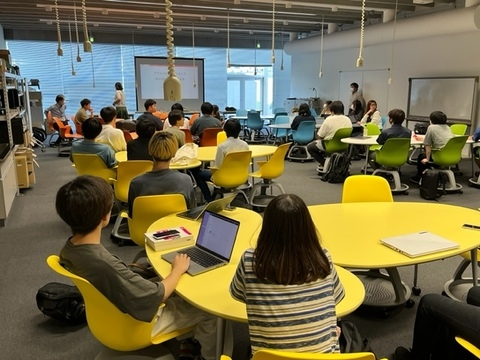
\includegraphics[width=8cm]{images/4.4.2_agilews.jpg}
    \caption{アジャイルワークショップの様子}
    \figlab{agilews}
\end{figure}
\bunseki{高橋慧流}

\section{GitHub勉強会}
私達はグループ内でGitHubの勉強会を行った．コミットやプッシュ，プル，フェッチなどの操作やリポジトリやブランチなどの用語についての知識を得た．また，危険な操作やエラーの対処法についてを学んだ．その後各自リポジトリを作成し，テスト用のFlutterプロジェクトでコミットやプッシュ，プルなどの基本的な操作を実践した．
\bunseki{南川虎之介}

\section{SCRUM BOOT CAMP THE BOOK スクラムチームではじめるアジャイル開発}
伊藤恵教授から書籍\wasyo{SCRUM BOOT CAMP THE BOOK スクラムチームではじめるアジャイル開発}\cite{scrumb}を借りた．この書籍はアジャイル開発について詳しく解説されており，時間があるときに読んで学んだ．特にスクラムというアジャイル開発の手法に焦点を当てている．本書を通じて，スクラムの基本的な役割であるプロダクトオーナーやスクラムマスターの役割や責任について理解を深めた．彼らの役割は，プロジェクトの成功に欠かせないものであり，それぞれがチームの効率性と成果の最大化を担っている．また，スクラムの始め方や見積もりの方法についても学んだ．スクラムでは，プロジェクトの開始時に適切なフレームワークを設定し，効果的なスプリントの計画と実行を行う．見積もりは，タスクの時間的な所要量を適切に評価するための重要なスキルであり，正確な見積もりを行うことでスプリントの進行管理が円滑になる．

\bunseki{高橋慧流}

\section{Flutter}
Flutter\footnote{https://flutter.dev}は，2018年にGoogleが正式リリースしたオープンソースのフレームワークである．Flutterが備える最大の特徴は，「iOSとAndroidのアプリを一度に開発できる」という点が挙げられる．加えて，Flutterは，ホットリロードに対応しているため高速開発が可能である．これらの理由から，Flutterによる開発を行っていくことに決めた．
\bunseki{南川虎之介}

\section{Firebase勉強会}
Firebase\footnote{https://firebase.google.com}勉強会はグループ内で夏季休暇で実施する予定である．
\bunseki{南川虎之介}

\section{API勉強会}
API勉強会はグループ内で夏季休暇で実施する予定である．
\bunseki{南川虎之介}
